% The Galois correspondence used in the proof of quadratic
% reciprocity: ℚ(ζ_q) over ℚ(√q*) over ℚ, matched with {1} ⊆ H ⊆ G.
% Source: book/tex/alg-NT/frobenius.tex (§ Application: Quadratic
% reciprocity, Step 1) — tikzcd.
\documentclass[border=2mm]{standalone}
\usepackage{tikz}
\usetikzlibrary{arrows.meta}
\usepackage{amssymb}
\usepackage{amsmath}
\begin{document}
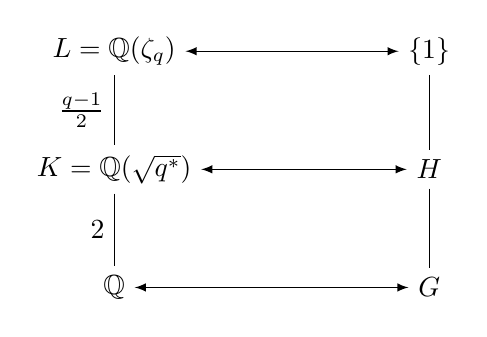
\begin{tikzpicture}[>=latex]
  \node (L)  at (0,3.0)   {$L = \mathbb{Q}(\zeta_q)$};
  \node (K)  at (0,1.5)   {$K = \mathbb{Q}(\sqrt{q^\ast})$};
  \node (Q)  at (0,0)     {$\mathbb{Q}$};
  \node (e)  at (4,3.0)   {$\{1\}$};
  \node (H)  at (4,1.5)   {$H$};
  \node (G)  at (4,0)     {$G$};
  \draw (L) -- (K) node[midway,left] {$\frac{q-1}{2}$};
  \draw (K) -- (Q) node[midway,left] {$2$};
  \draw (e) -- (H);
  \draw (H) -- (G);
  \draw[<->] (L) -- (e);
  \draw[<->] (K) -- (H);
  \draw[<->] (Q) -- (G);
\end{tikzpicture}
\end{document}
